\documentclass[8pt,landscape,a4paper,twoside]{extarticle}
\usepackage[utf8]{inputenc}
\usepackage[T1]{fontenc}
\usepackage{textcomp}
\usepackage{times}
\usepackage{multicol}
\usepackage[left=3mm, right=3mm, top=3mm, bottom=3mm, headheight=0mm, headsep=0mm, footskip=3mm, includefoot]{geometry}
\usepackage{enumitem}
\usepackage{amssymb}
\usepackage{scalerel}
\usepackage{xcolor}
\usepackage{tabularx}
\usepackage{hhline}
\usepackage{tikz}
\usepackage{listings}   % to use nodes inside listing see: https://texample.net/tikz/examples/tikz-listings/ 
\usepackage{hyperref}
\usepackage{tcolorbox}
\usepackage{anyfontsize}
\usepackage{ifthen}
\usepackage{calc}
\usepackage{draftwatermark}
\usepackage{contour}
\usepackage[normalem]{ulem}
\usepackage{fancyhdr}
\usepackage[explicit]{titlesec}
\usepackage{qrcode}



% tikz libraries
\usetikzlibrary{arrows, positioning}
\usetikzlibrary{arrows.meta, bending}
\usetikzlibrary{decorations.pathreplacing}
\usetikzlibrary{angles}
\usetikzlibrary{tikzmark}
\usetikzlibrary{petri}
\usetikzlibrary{positioning}
\usetikzlibrary{shapes}
\usetikzlibrary{calc}

\setlength{\columnsep}{1.5mm}       % column separation
\setlength{\columnseprule}{0.1pt}   % thickness of column separation line

% set document info
\def\title{Java für C++ Programmierer}
\def\dozent{Frieder Loch}
\def\semester{HS23}
\def\author{Laurin Heitzer}
\def\repo{https://github.com/P4ntomime/SumJavaCPP}

\hypersetup{hidelinks,
% set pdf metadata
pdfauthor={\author},
pdftitle={JavaC},
pdfsubject={\title{} \semester{}},
pdfkeywords={Gahn go lerne!!}}

\setcounter{secnumdepth}{0}        % no section numbering, remove if section numbering is needed

%% colors
\definecolor{mygray}{cmyk}{0,0,0,.45}
% \definecolor{Gray}{gray}{0.85}
\definecolor{sectioncolor}{HTML}{368d3f}

% color palette: https://colorkit.co/color-palette-generator/FF8552-9e22bd-404E7C-C32E15-225A28/
\definecolor{basegreen}{HTML}{225A28}
\definecolor{redcontrast}{HTML}{C32E15}
\definecolor{bluecontrast}{HTML}{404E7C}
\definecolor{coralcontrast}{HTML}{FF8552}
\definecolor{claretcontrast}{HTML}{9e22bd}

% colors for listings (code)
\definecolor{commentcolour}{HTML}{404E7C}
\definecolor{keywordcolour}{HTML}{225A28}
\definecolor{stringcolour}{HTML}{9e22bd}
\definecolor{numbercolour}{HTML}{808080}
\definecolor{backcolour}{HTML}{f5f5f0}


\setlength{\parindent}{0pt}        % no paragraph indentation
\setlist[enumerate]{label=\bfseries\arabic*., leftmargin=*, }   % enumerate style
\setlist[itemize]{leftmargin=1.5em}
\setlist{nosep}                    % no vertical spacing between list items

% scale ^ and _ in math mode
\catcode`_=\active% chktex 41 --> suppress ChkTeX warning
\catcode`^=\active% chktex 41
\newcommand_[1]{\ensuremath{\sb{\mathrm{\scaleobj{0.7}{#1}}}}}
\newcommand^[1]{\ensuremath{\sp{\mathrm{\scaleobj{0.7}{#1}}}}}

% inline tikz node for later referencing
\newcommand{\tikznode}[2]{% from https://tex.stackexchange.com/a/402466/121799
	\ifmmode%
	\tikz[remember picture,baseline= (#1.base),inner sep=0pt] \node(#1){$#2$};
	\else
	\tikz[remember picture,baseline= (#1.base),inner sep=0pt] \node(#1){#2};
	\fi}

% inline lst tikz node for later referencing
\newcommand{\lstnode}[2][0.5ex]{
	\tikz[overlay, remember picture, inner sep=0pt, yshift=#1, minimum width=0mm]\node(#2){};
}

% custom inline tcolorbox
\newtcbox{\mybox}
            [1]
            [backcolour]
            {on line,
            arc=0pt,
            outer arc=0pt,
            colback=#1,
            colframe=#1,
            boxsep=0pt,
            left=1pt,
            right=1pt,
            top=1pt,
            bottom=1pt,
            boxrule=0pt}

\makeatletter

% renew command for lstinputlisting with less vertical spacing
% \renewcommand{\lstinputlisting}[2][]{
%     \begingroup
%     \vspace{-0.6\abovedisplayskip}
%     \lst@setcatcodes%
%     \lst@inputlisting[#1]{#2}
%     \vspace{-0.6\abovedisplayskip}
% }

% custom text rightarrow to match tikz arrows
\renewcommand{\textrightarrow}{\tikz{\draw[-{Stealth[length=1.7mm]},double] (0,0) -- (0.3,0);}} % ChkTeX 8 --> suppress ChkTeX warning
\newcommand{\textlrarrow}{\tikz{\draw[{Stealth[length=1.7mm]}-{Stealth[length=1.7mm]},double] (0,0) -- (0.4,0);}} % ChkTeX 8 --> suppress ChkTeX warning

% custom command for size matched colored brackets
\newcommand{\bbr}[2]{\colorlet{saved}{.}\color{#1}\left(\color{saved}#2\color{#1}\right)\color{saved}}

% shortcuts for colored text
\newcommand{\cgn}[1]{{\color{basegreen}#1}}
\newcommand{\crd}[1]{{\color{redcontrast}#1}}
\newcommand{\cbl}[1]{{\color{bluecontrast}#1}}
\newcommand{\cor}[1]{{\color{coralcontrast}#1}}
\newcommand{\clt}[1]{{\color{claretcontrast}#1}}

% bullet command for items in tables
\newcommand\sbullet[1][.6]{\mathbin{\vcenter{\hbox{\scalebox{#1}{$\bullet$}}}}}
\newcommand{\tabitem}{~~\llap{\textbullet}~~}

% custom inline listings with box around them
\newcommand{\mylstbox}[2][columns=fullflexible]{\mybox{\lstinline[#1]{#2}}}
\newcommand{\mytclstbox}[2][columns=fullflexible]{\mybox{\lstinline[basicstyle=\sffamily\footnotesize\color{#1}, columns=fullflexible]{#2}}}

\newcommand\addvmargin[1]{
  \node[fit= (current bounding box),inner ysep=#1,inner xsep=0]{};
}

% stretch table rows
\renewcommand{\arraystretch}{1.2}

% custom underline command for exclusions on lowercase letters such as g, j, p, q, y
\renewcommand{\ULdepth}{1.75pt}
\contourlength{0.7pt}
\newcommand{\myul}[1]{%
  \uline{\phantom{#1}}%
  \llap{\contour*{white}{#1}}%
}

% define page numbering style (bottom right on odd pages, bottom left on even pages)
\pagestyle{fancy}
\fancyhf{} % clear all header and footer fields
\renewcommand{\headrulewidth}{0pt}
\renewcommand{\footrulewidth}{0pt}
\fancyfoot[LE,RO]{\tikz{\node[fill=basegreen, node font=\bfseries, text=white, minimum width=6mm, minimum height=3mm, inner sep=0mm, align=center]{\thepage};}}


% custom title formats
\titleformat{\section}
            {\fontsize{9}{8}\selectfont\bfseries}
            {\thesection}
            {0mm}
            {\colorbox{lightgray!40}{\rule[-.2\baselineskip]{0pt}{2.5mm}\parbox{\dimexpr\columnwidth-2\fboxsep\relax}{\textcolor{sectioncolor}{#1}}}}
\titlespacing{\section}
             {0mm}
             {.2ex}
             {.2ex}
\titleformat{\subsection}
            {\fontsize{9}{8}\selectfont\bfseries}
            {\thesubsection}
            {0mm}
            {\phantomsection\myul{#1}} % \phantomsection to make hyperref link to correct section
\titlespacing{\subsection}
             {0mm}
             {1ex}
             {.2ex}
\renewcommand{\subsubsection}{\@startsection{subsubsection}{1}{0mm}%
                                {.2ex}%
                                {.2ex}%x
                                {\color{mygray}\normalsize\bfseries}}

% custom pagelimit command. source: https://stackoverflow.com/questions/2720534/force-a-maximum-number-of-pages-in-latex 
% colors all pages after the specified limit red
\newcounter{pagecount}
\newcommand{\limitpages}[1]{
    \setcounter{pagecount}{0}%
    \gdef\maxpages{#1}%
    \ifx\latex@outputpage\@undefined\relax%
        \global\let\latex@outputpage\@outputpage%
    \fi%
    \gdef\@outputpage{%
        \addtocounter{pagecount}{1}%
        \ifnum\value{pagecount}>\maxpages\relax%
            % Do not output the page
            \SetWatermarkText{#1 Seiten Limit erreicht!}%
            \SetWatermarkScale{0.35}%
            \pagecolor{red}
            \latex@outputpage%
        \else%
            \SetWatermarkText{}%
            \latex@outputpage%
        \fi%
    }%
}

\limitpages{6}  % set page limit to 6 pages


% hack to fix asterisk in lstlisting
\lst@CCPutMacro%
    \lst@ProcessOther{"2A}{%
         {\raisebox{0.125pt}{*}}}
    \@empty\z@\@empty%

\makeatother

% listings style (code)
\lstdefinestyle{mystyle}{
    backgroundcolor=\color{backcolour},   
    commentstyle=\color{commentcolour},
    keywordstyle=\bfseries\color{keywordcolour},
    numberstyle=\tiny\color{numbercolour},
    stringstyle=\color{stringcolour},
    basicstyle=\sffamily,
    breakatwhitespace=false,
    breaklines=true,
    captionpos=b,
    keepspaces=true,
    numbers=left,
    numbersep=2pt,
    showspaces=false,
    showstringspaces=false,
    showtabs=false,
    aboveskip=0pt,
    belowskip=0pt,
    float=*,
    tabsize=4,
	xleftmargin=1em,
	language=Java,
    extendedchars=true,
    inputencoding=cp1252,
	columns=[l]fullflexible	% see: https://tex.stackexchange.com/questions/99416/latex-source-code-listing-with-less-space-between-characters or manual
}

% custom lstinline command with custom colors
\def\purplst{\begingroup\color{claretcontrast}}
\def\greenlst{\begingroup\color{basegreen}}
\def\redlst{\begingroup\color{redcontrast}}
\def\ywlst{\begingroup\color{coralcontrast}}
\def\bluelst{\begingroup\color{bluecontrast}}
\def\endlstcol{\endgroup}

% basic lstinline style without colors
\lstdefinestyle{basestyle}{
    backgroundcolor=\color{backcolour},
    keywordstyle=\bfseries,
    numberstyle=\tiny\color{numbercolour},
    basicstyle=\sffamily\footnotesize,
    breakatwhitespace=false,     
    breaklines=true,
    captionpos=b,
    keepspaces=true,
    numbers=none,
    numbersep=2pt,
    showspaces=false,
    showstringspaces=false,
    showtabs=false,
    tabsize=4,
    xleftmargin=0em,
    language=Java,
    columns=flexible,	% see: https://tex.stackexchange.com/questions/99416/latex-source-code-listing-with-less-space-between-characters or manual
}

\lstset{
    style=mystyle,
    morekeywords={final, override, enum, var, List, Set, Map, String, Object},
    moredelim=[il][\textcolor{coralcontrast}]{¦¦},
    moredelim=[is][\textcolor{coralcontrast}]{&&}{&&},
    moredelim=[is][\textcolor{claretcontrast}]{@}{@},
}


\begin{document}
	\begin{multicols*}{3}
		\begin{minipage}[c]{0.125\columnwidth}
    \centering%
    \qrcode[level=L, version=0,height=0.9\columnwidth]{https://github.com/P4ntomime/SumJavaCPP}
\end{minipage}\hfill%
\begin{minipage}[c]{0.83\columnwidth}
    \makeatletter
	\begin{tabular}{l}
		{\Large\bfseries\@title{} --- \dozent{}}\\
		\@author\\
		{\small \semester}
	\end{tabular}
    \makeatother
\end{minipage}
        \section{Java Virtual Machine}
\subsection{Java Runtime-Architektur}

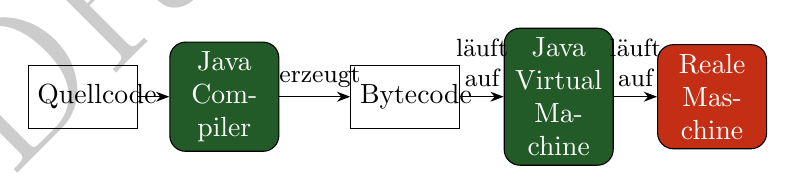
\begin{tikzpicture}[
    every node/.style={
        draw=black, 
        minimum height=0.8cm,
        minimum width=1.15cm,
        text width=1.15cm,
        align=center},
    >=Stealth]
    \node (srccode) {Quellcode};
    \node[fill=basegreen, text=white, right=0.4cm of srccode, rounded corners=0.2cm] (javac) {Java Compiler};
    \node[right=0.9cm of javac] (bytecode) {Bytecode};
    \node[fill=basegreen, text=white, right=0.55cm of bytecode, rounded corners=0.2cm] (jvm) {Java Virtual Machine};
    \node[fill=redcontrast, text=white, right=0.55cm of jvm, rounded corners=0.2cm] (os) {Reale Maschine};

    \begin{scope}[
        every node/.style={
            draw=none, 
            minimum height=0.3cm, 
            minimum width=0.3cm, 
            align=center, 
            text width=0.9cm,
            font=\small}]
        \draw[->] (srccode) -- (javac);
        \draw[->] (javac.east) to node[midway, above] {erzeugt} (bytecode.west);
        \draw[->] (bytecode) to node[midway, above] {läuft\\ auf} (jvm);
        \draw[->] (jvm) to node[midway, above] {läuft\\ auf} (os);
    \end{scope}
\end{tikzpicture}

\subsection{Bytecode}
\begin{minipage}{0.25\columnwidth}
    \lstinputlisting[style=basestyle, xleftmargin=1em, numbers=left, escapechar=!]{snippets/bytecode.java}
\end{minipage}\hfill
\begin{minipage}{0.71\columnwidth}
    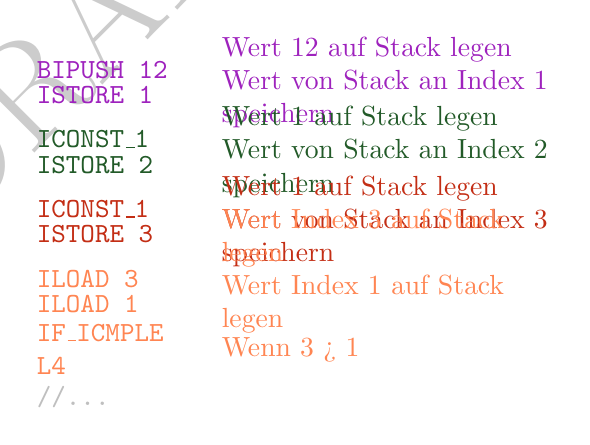
\begin{tikzpicture}[every node/.style={draw=none, align=flush left, text width=2.1cm, minimum height=0.1cm}]
        \node[text=claretcontrast] (0) {\texttt{BIPUSH 12}\\\vspace{-1mm}\texttt{ISTORE 1}};
        \node[right=0cm of 0, text=claretcontrast, text width=4.2cm] {Wert 12 auf Stack legen\\Wert von Stack an Index 1 speichern};

        \node[below=0.1cm of 0, text=basegreen] (1) {\texttt{ICONST\_1}\\\vspace{-1mm}\texttt{ISTORE 2}};
        \node[right=0cm of 1, text=basegreen, text width=4.2cm] {Wert 1 auf Stack legen\\Wert von Stack an Index 2 speichern};

        \node[below=0.1cm of 1, text=redcontrast] (2) {\texttt{ICONST\_1}\\\vspace{-1mm}\texttt{ISTORE 3}};
        \node[right=0cm of 2, text=redcontrast, text width=4.2cm] {Wert 1 auf Stack legen\\Wert von Stack an Index 3 speichern};
        
        \node[below=0.1cm of 2, text=coralcontrast] (3) {\texttt{ILOAD 3}\\\vspace{-1mm}\texttt{ILOAD 1}};
        \node[below=-1mm of 3, text=coralcontrast] (3a) {\texttt{IF\_ICMPLE L4}};
        \node[right=0cm of 3a, text=coralcontrast, text width=4.2cm] (3acomment) {Wenn 3 > 1};
        \node[above=-2mm of 3acomment, text=coralcontrast, text width=4.2cm] (3b) {Wert Index 3 auf Stack legen\\Wert Index 1 auf Stack legen};
        \node[below=-1mm of 3a, text=lightgray] (4) {\texttt{//\ldots}};
    \end{tikzpicture}
\end{minipage}


\begin{minipage}[t]{0.36\columnwidth}
    \subsubsection{Java Bytecode}
    \raggedright%
    \begin{itemize}
        \item Standardisierte Zwischensprache
        \item Für hypot. Stackmaschine
    \end{itemize}
\end{minipage}\hfill%
\begin{minipage}[t]{0.63\columnwidth}
    \subsubsection{Java Virtual Machine}
    \raggedright%
    \begin{itemize}
        \item Interpretiert Bytecode
        \item Implementiert für jede Zielplattform
        \item \textbf{J}ust-\textbf{I}n-\textbf{T}ime Compiler in realen Maschinencode
    \end{itemize}
\end{minipage}
        \section{Datentypen}
\subsection{Primitive Datentypen}
\begin{itemize}
    \item Im Gegensatz zu C++ sind Wertebereiche auf jeder Plattform gleich
    \item Keine \texttt{unsigned} Typen
\end{itemize}

\begin{center}
    \begin{tabularx}{0.82\columnwidth}{@{}c l l@{}}
        \lstinline{boolean}    & Boolscher Wert        & true, false\\\hline
        \lstinline{char}       & Textzeichen (UTF16)   & 'a', 'b', 'c'\\\hline
        \lstinline{byte}       & Ganzzahl (8 Bit)             & -128 bis 127\\\hline
        \lstinline{short}      & Ganzzahl (16 Bit)             & -32'768 bis 32'767\\\hline
        \lstinline{int}        & Ganzzahl (32 Bit)             & -2^{31} bis 2^{31}-1\\\hline
        \lstinline{long}       & Ganzzahl (64 Bit)             & -2^{63} bis 2^{63}-1, 1L (L Suffix)\\\hline
        \lstinline{float}      & Gleitkommazahl (32 Bit)       & 0.1f, 2e4f (2*10^4)\\\hline
        \lstinline{double}     & Gleitkommazahl (64 Bit)       & 0.1, 2e4 (2*10^4)\\
    \end{tabularx}
\end{center}

\subsection{Typumwandlung}
\begin{minipage}{0.6\columnwidth}
    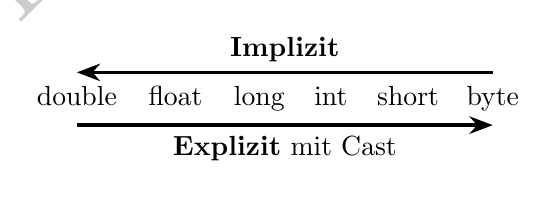
\begin{tikzpicture}[every node/.style={draw=none}]
        \node (double) {\strut\lstinline{double}};
        \node[right=0.1cm of double] (float) {\strut\lstinline{float}};
        \node[right=0.1cm of float] (long) {\strut\lstinline{long}};
        \node[right=0.1cm of long] (int) {\strut\lstinline{int}};
        \node[right=0.1cm of int] (short) {\strut\lstinline{short}};
        \node[right=0.1cm of short] (byte) {\strut\lstinline{byte}};
        \draw[-{Stealth}, very thick] (double.south) to node[below] {\textbf{Explizit} mit Cast} (byte.south);
        \draw[-{Stealth}, very thick] (byte.north) to node[above] {\textbf{Implizit}} (double.north);
    \end{tikzpicture}
\end{minipage}
\begin{minipage}{0.35\columnwidth}
    Boolean kann nicht implizit in andere Typen umgewandelt werden.
\end{minipage}

\subsubsection{Explizite Typumwandlung}
Beispiel: \mylstbox{int i = (int) 3.14;}\hfill\newline
Informationsverlust:
\begin{itemize}
    \item Ganzzahl \textrightarrow{} Ganzzahl: Nur untere Bits werden übernommen
    \item Gleitkommazahl \textrightarrow{} Ganzzahl: Nachkommastellen werden abgeschnitten
\end{itemize}

\subsection{Arrays}
\begin{itemize}
    \item Speichern Referenzen auf gleichartige Objekte
    \item Zugriff über Index
\end{itemize}
Beispiel: \mylstbox{int[] a = new int[5];} \tikz[remember picture, overlay, x=5mm, y=5mm]{
    \foreach\x in {0,1,...,4}{
        \node[draw,fill=basegreen, text=white, minimum width=5mm] at ($(\x,0) + (6,0.25)$) (a) {0};
        \node[draw=none, above=0mm of a] {\sffamily\normalsize a[\x]};}}\hfill\null\\
Wenn Arrays vergrössert werden, wird deren Inhalt in einen neuen, grösseren Speicherbereich kopiert.

\subsubsection{Mehrdimensionale Arrays}
Beispiel: \mylstbox{int&&[]&&@[]@ m = new int&&[2]&&@[3]@;}\tikz[baseline=1ex, remember picture, overlay, x=5mm, y=3.75mm]{
    \foreach\x in {0,1,2}{
        \node[draw=none] at ($(\x,-1) + (7,0)$) (a) {\clt{\x}};
        \foreach\y in {0,1}{
            \ifthenelse{\x=0}{\node[draw=none] at ($(0,{1-\y}) + (6,0)$) (a) {\cor{\y}};}{}%
            \node[draw,fill=basegreen, text=white, minimum width=5mm] at ($(\x,\y) + (7,0)$) (a) {0};}}
    \node[draw=none, anchor=east] at (5.75,0.5) {\cor{Erster Index}};
    \node[draw=none, anchor=north] at (8, -1.25) {\clt{Zweiter Index}};
    }\vspace{2mm}\newline
\mylstbox{m.length} \textrightarrow{} 2 \qquad \mylstbox{m[0].length} \textrightarrow{} 3
\vspace{3mm}

\subsection{Einordnung}
\begin{center}
    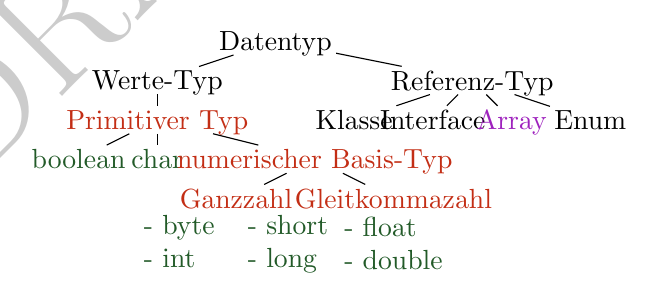
\begin{tikzpicture}[>={Stealth}, every node/.style={inner sep=0.5mm,text depth=0}]
        \node (dt) at (0,0) {Datentyp};
        \node (wt) at (-1.5,-0.5) {Werte-Typ};
        \node (rt) at (2.5,-0.5) {Referenz-Typ};
        \node (kl) at (1,-1) {Klasse};
        \node (in) at (2,-1) {Interface};
        \node (ar) at (3,-1) {\color{claretcontrast}Array};
        \node (en) at (4,-1) {Enum};
        \node (pt) at (-1.5,-1) {\color{redcontrast}Primitiver Typ};
        \node (bo) at (-2.5,-1.5) {\color{basegreen}boolean};
        \node (ch) at (-1.5,-1.5) {\color{basegreen}char};
        \node (nt) at (0.5,-1.5) {\color{redcontrast}numerischer Basis-Typ};
        \node (gz) at (-0.5,-2) {\color{redcontrast}Ganzzahl};
        \node (glz) at (1.5,-2) {\color{redcontrast}Gleitkommazahl};
        \renewcommand{\arraystretch}{1.2}
        \node[below=-0.8mm of gz, align=flush left, minimum width=2cm] {\begingroup\color{basegreen}\renewcommand{\arraystretch}{1}\begin{tabular}{@{}l l@{}}- byte &- short\\- int&- long\end{tabular}\endgroup};
        \node[below=0mm of glz, align=flush left, minimum width=2cm] {\color{basegreen}- float\\\color{basegreen}- double};
        \draw (dt) -- (wt);
        \draw (dt) -- (rt);
        
        \draw (wt) -- (pt);
        
        \draw (rt) -- (kl);
        \draw (rt) -- (in);
        \draw (rt) -- (ar);
        \draw (rt) -- (en);
        
        \draw (pt) -- (bo);
        \draw (pt) -- (ch);
        \draw (pt) -- (nt);
        
        \draw (nt) -- (gz);
        \draw (nt) -- (glz);
        
    \end{tikzpicture}
\end{center}\vspace{-\belowdisplayskip}
        \section{Enums}
Enums sind ein eigener Datentyp, mit endlichem Wertebereich.
\subsection{Syntax}
\vspace{-0.8\abovedisplayskip}
\begin{minipage}[t]{0.49\columnwidth}
    \subsubsection{Definition}
    \lstinputlisting{snippets/enum.java}
\end{minipage}\hfill
\begin{minipage}[t]{0.49\columnwidth}
    \subsubsection{Verwendung}
    \lstinputlisting{snippets/enum2.java}
\end{minipage}
Enums kann man auch als eine Art Klasse interpretieren. Sie können auch Methoden, Variablen und Konstruktoren enthalten. 
Zusätzlich sind sie auch \textit{type-safe}.\\
Es ist auch möglich einzelnen Enum-Konstanten Werte zuzuweisen:
\lstinputlisting{snippets/enum3.java}

        \section{ArrayList}
\subsection{Eigenschaften}
\begin{itemize}
    \item ArrayList enthält Referenzen auf Objekte
    \item Kann dynamisch vergrössert/verkleinert werden
    \item Kann nicht direkt mit primitiven Datentypen (\lstinline{int}, \lstinline{float}, etc.) verwendet werden
\end{itemize}

\subsection{Syntax}
\mylstbox{var stringList = new ArrayList<String>();}

\subsection{Wrapping}
Um einen Primitiven Datentyp zu referenzieren, muss dieser zuerst in ein Objekt gewrappt werden.
Boxing/Unboxing implizit möglich.
\vspace{-0.8\abovedisplayskip}
\begin{center}
    \begin{tabularx}{0.45\columnwidth}{@{}l l@{}}
        \textbf{Primitiver Typ} & \textbf{Wrapper-Klasse}\\\hhline{==}
        \lstinline{boolean} & \lstinline{Boolean}\\\hhline{--}
        \lstinline{char} & \lstinline{Character}\\\hhline{--}
        \lstinline{byte} & \lstinline{Byte}\\\hhline{--}
        \lstinline{short} & \lstinline{Short}\\
    \end{tabularx}
    \begin{tabularx}{0.45\columnwidth}{@{}l l@{}}
        \textbf{Primitiver Typ} & \textbf{Wrapper-Klasse}\\\hhline{==}
        \lstinline{int} & \lstinline{Integer}\\\hhline{--}
        \lstinline{long} & \lstinline{Long}\\\hhline{--}
        \lstinline{float} & \lstinline{Float}\\\hhline{--}
        \lstinline{double} & \lstinline{Double}\\
    \end{tabularx}
\end{center}
    
\subsection{Weitere Collections}
\begin{tabular}{@{}l l@{}}
    \lstinline!List! &Folge von Elementen\\
    \lstinline!Set! &Menge von Elementen\\
    \lstinline!Map! &Abbildung von Schlüssel auf Wert
\end{tabular}

        \section{Methoden}
% TODO: tbd
\subsection{Aufruf}\vspace{-2mm}
\begin{minipage}[t]{0.49\columnwidth}
    \subsubsection{Aufruf ohne Argumente}
    \mylstbox{starLine();}
\end{minipage}
\begin{minipage}[t]{0.5\columnwidth}
    \subsubsection{Aufruf mit Argumenten}
    \mylstbox{symbolLine('*', 5);}
\end{minipage}

\subsection{Call by Value}
\begin{itemize}
    \item Wert des Arguments wird in Parameter kopiert
    \item Änderung der Parameter ausserhalb Funktion nicht sichtbar
\end{itemize}

\subsubsection{Mit Referenztypen}
Referenz des Arguments wird in Parameter kopiert.
\begin{itemize}
    \item Änderung am Objekt sichtbar
    \item Änderung an der Referenz nicht sichtbar
\end{itemize}\vspace{-3mm}
\begin{minipage}[t]{0.49\columnwidth}
    \lstinputlisting{snippets/callbyvalref.java}
\end{minipage}\hfill
\begin{minipage}[t]{0.5\columnwidth}
    \lstinputlisting{snippets/callbyvalref2.java}
\end{minipage}

\subsection{Deklaration}
\vspace{-2mm}
\begin{minipage}[t]{0.49\columnwidth}
    \subsubsection{Deklaration ohne Parameter}
    \lstinputlisting{snippets/method.java}
\end{minipage}\hfill
\begin{minipage}[t]{0.5\columnwidth}
    \subsubsection{Deklaration mit Parameter}
    \lstinputlisting{snippets/method2.java}
\end{minipage}

\subsection{Rückgabewert}
\lstinline{return}-Anweisung zwingend, ausnahme: \lstinline{void}-Methoden

\subsection{Modifiers (gelten auch für Klassen und Variablen)}
\begin{itemize}
    \item \lstinline{public}: von überall aus sichtbar
    \item \lstinline{private}: nur innerhalb der Klasse sichtbar
    \item \lstinline{protected}: nur innerhalb der Klasse und von Subklassen sichtbar
    \item \lstinline{static}: Methode gehört zur Klasse, nicht zu einem Objekt (Instanziierung der Klasse nicht nötig)
    \item \lstinline{final}: Methode kann nicht überschrieben werden
    \item \lstinline{abstract}: Methode muss in Subklasse überschrieben werden
\end{itemize}

        \section{Variadische Methoden}
Variadische Methoden sind Methoden, die eine variable Anzahl an Argumenten akzeptieren.
\subsection{Syntax}
\vspace{-0.8\abovedisplayskip}
\begin{minipage}[t]{0.49\columnwidth}
    \subsubsection{Definition}
    \lstinputlisting{snippets/variadisch.java}
\end{minipage}\hfill
\begin{minipage}[t]{0.49\columnwidth}
    \subsubsection{Aufruf}
    \lstinputlisting{snippets/variadisch2.java}
\end{minipage}
\begin{itemize}
    \item Compiler erzeugt für variable Parameter ein Array, welches die Argumente enthält.
    \item Argumente können jeweils nur von \textbf{einem} Typ sein.
    \item Parameter in der Variadischen Funktion muss \textbf{immer} der letzte Parameter sein.
    \item Parameter kann auch als Array übergeben werden.
\end{itemize}
        \section{Klassen}
\subsection{Definition}
Eine Klasse spezifiziert die Gemeinsamkeiten einer Menge von Objekten mit denselben Eigenschaften, 
demselben Verhalten und denselben Beziehungen. [Balzert]

\begin{minipage}[t]{0.5\columnwidth}
    \subsection{Aufbau}
    % \vspace{-2mm}
    \lstinputlisting{snippets/klasse.java}
\end{minipage}\hfill%
\begin{minipage}[t]{0.49\columnwidth}
    \subsubsection{Konstruktor}
    \raggedright%
    \begin{itemize}
        \item Initialisiert ein Objekt/eine Klasse
        \item Hat keinen Rückgabewert
        \item Hat gleichen Namen wie Klasse
        \item Kann überladen werden
        \item Compiler erzeugt einen Standardkonstruktor, wenn kein Konstruktor definiert ist
    \end{itemize}
\end{minipage}

\begin{minipage}[t]{0.41\columnwidth}
    \subsection{\textsf{\textbf{\textcolor{keywordcolour}{null}}}-Referenz}
    \raggedright%
    \begin{itemize}
        \item Referenz auf "kein Objekt"
        \item Meist zur Initialisierung von Referenzen verwendet
        \item Gültig für alle Referenztypen
        \item Dereferenzierung führt zu \lstinline{NullPointerException}
    \end{itemize}
\end{minipage}\hfill%
\begin{minipage}[t]{0.59\columnwidth}
    \raggedright%
    \subsection{Selbstreferenz}
    Zur Selbstreferenz wird das Schlüsselwort \lstinline{this} verwendet.
    
    \subsection{Instanziierung}
    Objekte werden mit dem \lstinline{new}-Operator erzeugt (instanziiert): \mylstbox{Rectangle r = new Rectangle();}
\end{minipage}


        \section{Binding}
Bei Referenzen wird zwischen statischem und dynamischem Binding unterschieden.
% \vspace{-0.7\abovedisplayskip}
\begin{lstlisting}[numbers=none, 
    escapechar=!, 
    xleftmargin=-3mm, 
    linewidth=0.39\columnwidth,
    framexleftmargin=-3mm]
    Vehi!\tikz[overlay, remember picture]\node[xshift=-0.5mm,yshift=-0.5mm](statnode){};!cle vehicle = new Ca!\tikz[overlay, remember picture]\node[xshift=-0.5mm,yshift=-0.5mm](dynnode){};!r();
\end{lstlisting}
\begin{tikzpicture}[remember picture, overlay]
    \node[anchor=west] (t2) at (3.9,0.2) {Dynamischer Typ};
    \node[anchor=west] (t1) at (6.1,-0) {Statischer Typ};
    \draw[rounded corners=2pt,-{Stealth}] (t1.west) -| (statnode);
    \draw[rounded corners=1pt,-{Stealth}] (t2.west) -| (dynnode);
\end{tikzpicture}

\subsection{Statische Bindung}
\vspace{-0.8\abovedisplayskip}
\begin{minipage}[t]{0.59\columnwidth}
    \lstinputlisting{snippets/sbinding1.java}
\end{minipage}\hfill%
\begin{minipage}[t]{0.4\columnwidth}
    \lstinputlisting{snippets/sbinding2.java}
\end{minipage}

\begin{minipage}[t]{0.52\columnwidth}
    \subsection{Dynamische Bindung}
    \raggedright%
    Bei Aufruf nicht-privater Instanzmethoden wird Methode gemäss dynamischem Typ des Objekts aufgerufen.
    \lstinputlisting{snippets/dbinding1.java}
    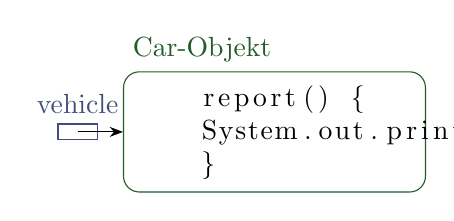
\begin{tikzpicture}
        \node[draw=bluecontrast, minimum width=0.5cm, minimum height=0.2cm, inner sep=0mm] (v) at (0.5,-2) {};
        \node[text=bluecontrast, above=0mm of v] {vehicle};
        \node[draw=basegreen, rounded corners=2mm, text width=3.6cm, align=center] (co) at (3,-2) {\begin{lstlisting}[numbers=none,
            xleftmargin=0.1mm,
            xrightmargin=0.1mm,
            linewidth=\columnwidth,
            framexleftmargin=0mm,
            framextopmargin=0mm,
            framexbottommargin=0mm,
            aboveskip=-1mm,
            belowskip=0mm,
            backgroundcolor=\color{white}]
    report() {
    System.out.println("Car");
    }\end{lstlisting}};
        \node[text=basegreen, above=0mm of co.north west, anchor=south west] {Car-Objekt};
        \draw[-{Stealth}] (v.center) -- (co.west);
    \end{tikzpicture}
\end{minipage}\hfill%
\begin{minipage}[t]{0.45\columnwidth}
    \subsection{Details}
    \subsubsection{Statische Bindung bei\ldots}
    \begin{itemize}
        \item \ldots Konstruktoren
        \item \ldots privaten Methoden
        \item \ldots statischen Methoden
    \end{itemize}
    
    \subsubsection{Dynamische Bindung bei\ldots}
    \begin{itemize}
        \item \ldots nicht-privaten Instanzmethoden
    \end{itemize}
\end{minipage}

        \section{Vererbung}

\begin{minipage}[t]{0.5\columnwidth}
    \subsection{Syntax}
    \lstinputlisting{snippets/vererbung.java}
    \subsection{Vererbung in Java}
    \begin{itemize}
        \item Subklassen erben alle Attribute und Methoden aller Superklassen, die nicht \lstinline{private} sind.
    \end{itemize}
\end{minipage}\hfill
\begin{minipage}[t]{0.46\columnwidth}
    \subsection{Vererbungshierarchie}
    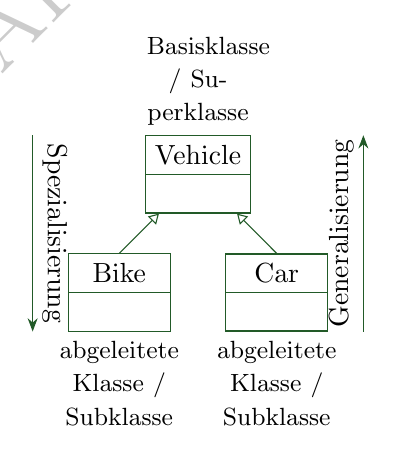
\begin{tikzpicture}[>=Stealth, draw=none]
        \begin{scope}[every node/.style={
            rectangle split,
            rectangle split parts=2, 
            draw=basegreen, 
            minimum width=1.3cm, 
            minimum height=2cm}]
            \node (v) at (0,0) {Vehicle \nodepart{two}\phantom{V}};
            \node (c) at (1,-1.5) {Car \nodepart{two}\phantom{V}};
            \node (b) at (-1,-1.5) {Bike \nodepart{two}\phantom{V}};
        \end{scope}
        \node[above=0mm of v, text width=1.3cm, align=center] {\small Basisklasse / Superklasse};
        \node[below=0mm of c, text width=2cm, align=center] {\small abgeleitete Klasse / Subklasse};
        \node[below=0mm of b, text width=2cm, align=center] {\small abgeleitete Klasse / Subklasse};
        \draw[-{Triangle[open]}, draw=basegreen] (c.north) -- (v);
        \draw[-{Triangle[open]}, draw=basegreen] (b.north) -- (v);
        \draw[->, draw=basegreen] ({(-2.1,-0.5)} |- v.north west) to node[above, rotate=-90, align=center]{Spezialisierung} ({(-2.1,-0.5)} |- c.south west);
        \draw[->, draw=basegreen] ({(2.1,-0.5)} |- b.south east) to node[above, rotate=90, align=center]{Generalisierung} ({(2.1,-0.5)} |- v.north east);
    \end{tikzpicture}
\end{minipage}



\subsection{Object}
Alle Klassen erben implizit von der Klasse \lstinline{Object}. Diese stellt folgende Methoden zur Verfügung:
\begin{itemize}
    \item \lstinline{public boolean equals(Object obj)}: Vergleicht zwei Objekte auf Gleichheit
    \item \lstinline{public String toString()}: Gibt eine String-Repräsentation des Objekts zurück
    \item \lstinline{public int hashCode()}: Gibt einen Hashcode für das Objekt zurück
\end{itemize}
Diese Methoden können in jeder Klasse überschrieben werden, um sie an die jeweiligen Bedürfnisse anzupassen.

\subsection{Polymorphie}

\begin{minipage}[t]{0.65\columnwidth}
    Ein Objekt ist mit seinem Typ, sowie Typen aller Superklassen kompatibel. Jedoch nicht mit Typen von Subklassen.
\end{minipage}\hfill%
\begin{minipage}[t]{0.34\columnwidth}
    \begin{itemize}
        \item \mylstbox{Car c = new Car();}
        \item \mylstbox{Vehicle v = c;}
        \item \mylstbox{Object o = v;}
    \end{itemize}
\end{minipage}

\subsubsection{Overriding}
\vspace{-0.7\abovedisplayskip}
\begin{minipage}[t]{0.5\columnwidth}
    \lstinputlisting{snippets/overriding1.java}
\end{minipage}
\begin{minipage}[t]{0.49\columnwidth}
    \lstinputlisting{snippets/overriding2.java}
\end{minipage}
\begin{itemize}
    \item Methoden können in Subklassen überschrieben werden
    \item Signatur \textbf{muss} gleich sein
    \item \lstinline{¦¦@Override} Annotation ist optional, aber empfohlen
    \item Falls eine Klasse eine Superklasse, sowie ein Interface implementieren/erweitern soll, so muss zuerst \lstinline{extends} \textit{SuperKlasse} und dann \lstinline{implements} \textit{Schnittstelle} stehen (mit Leerzeichen dazwischen, kein Komma).
\end{itemize}

        \section{Schnittstellen}


\subsection{Syntax}
\begin{minipage}[t]{0.51\columnwidth}
    \raggedright%
    \begin{itemize}
        \item Implizit \lstinline{public} und \lstinline{abstract}. (Andere Modifikatoren nicht erlaubt)
        \item Alle Methoden müssen von der implementierenden Klasse implementiert werden, sofern diese nicht \lstinline{abstract} ist.
        \item Methoden dürfen keine Implementierung im Interface haben.
        \item Interfaces können nicht instanziiert werden.
        \item Eine Implementierung kann mehrer Interfaces implementieren.
        \item Falls mehrere Methoden mit gleichem Namen existieren, wird nur eine Methode implementiert.
        \item Konstanten werden automatisch als \lstinline{public static final} deklariert.
    \end{itemize}
\end{minipage}\hfill%
\begin{minipage}[t]{0.48\columnwidth}
    \vspace{-0.8\abovedisplayskip}
    \lstinputlisting{snippets/interface1.java}
    \lstinputlisting{snippets/interface2.java}
\end{minipage}


% \begin{minipage}[t]{0.51\columnwidth}
%     \raggedright%
%     \begin{itemize}
%         \end{itemize}
% \end{minipage}\hfill%
% \begin{minipage}[t]{0.48\columnwidth}
%     \vspace{-0.8\abovedisplayskip}
% \end{minipage}
% ugly workaround to use less space
% FIXME: find a better solution
\begin{itemize}
    \item Falls mehrere Konstanten mit demselben Namen existieren, muss der Name des Interfaces vorangestellt werden.
    \item Schnittstellen können andere Schnittstellen erweitern mit \lstinline{extends}.
\end{itemize}


\subsection{Lose Kopplung}
Mittels loser Kopplung können mehrere Teams einfach miteinander arbeiten. 
Die Teams müssen sich nur auf die Schnittstelle einigen. 
Die Implementierung kann unabhängig voneinander erfolgen.

\begin{minipage}[t]{0.52\columnwidth}
    \subsection{Abstrakte Klassen}
    Klasse, die nicht instanziiert werden kann und mindestens eine abstrakte Methode enthält.
\end{minipage}\hfill
\begin{minipage}[t]{0.45\columnwidth}
    \subsection{Abstrakte Methoden}
    Deklaration einer Methode ohne Implementierung. Geht nur in abstrakten Klassen und Interfaces.
    \lstinputlisting{snippets/abstractmethod.java}
\end{minipage}

\vspace{-7mm}
\subsection{Set-Interface}
Menge von Elementen ohne Duplikate.
\subsubsection{Methoden}
\begin{itemize}
    \item \lstinline{boolean add(E e)}: Fügt Element hinzu, wenn nicht bereits vorhanden
    \item Gleichheitsprüfung mit \lstinline{equals()}
\end{itemize}

\subsubsection{Beispiel}
\lstinputlisting{snippets/set.java}
\subsection{Map-Interface}
\begin{itemize}
    \item Objekt, das Schlüssel auf Werte abbildet.
    \item Kann keine Duplikate von Schlüsseln enthalten.
    \item Jeder Schlüssel kann höchstens einem Wert zugeordnet werden.
\end{itemize}
\begin{minipage}[t]{0.31\columnwidth}
    \subsubsection{Visualisierung}
    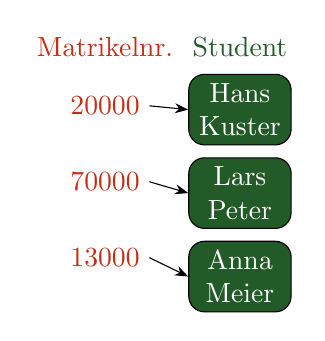
\begin{tikzpicture}[every node/.style={align=center}, >=Stealth]
        \def\deltay{1.5mm}
        \def\minheight{8mm}
        \begin{scope}[every node/.style={text=redcontrast, minimum height=\minheight}]
            \node[minimum height=0.2cm] (keyname) at (0,0) {Matrikelnr.};
            \node[below=1mm of keyname] (key1) {20000};
            \node[below=\deltay of key1] (key2) {70000};
            \node[below=\deltay of key2] (key3) {13000};
        \end{scope}
        \begin{scope}[every node/.style={align=center,fill=basegreen, text=white, draw, rounded corners=2mm, minimum width=1.3cm, minimum height=\minheight}]
            \node[minimum height=0.2cm,fill=none,draw=none,text=basegreen,right=0mm of keyname] (valuename) {Student};
            \node[below=1mm of valuename] (value1) {Hans\\ Kuster};
            \node[below=\deltay of value1] (value2) {Lars\\ Peter};
            \node[below=\deltay of value2] (value3) {Anna\\ Meier};
        \end{scope}
        \draw[->] (key1.east) -- (value1.west);
        \draw[->] (key2.east) -- (value2.west);
        \draw[->] (key3.east) -- (value3.west);
    \end{tikzpicture}    
\end{minipage}\hfill
\begin{minipage}[t]{0.69\columnwidth}
    \subsubsection{Beispiel}
    \phantom{t}\vspace{-3mm}
    \lstinputlisting[inputencoding=cp1252]{snippets/map.java} % map.java needs to be saved with Windows 1252 (cp1252) encoding!
\end{minipage}

\subsection{Comparator-Interface}
\vspace{-0.8\abovedisplayskip}
\begin{minipage}[t]{0.45\columnwidth}
    \lstinputlisting{snippets/compintf.java}
\end{minipage}
\begin{minipage}[t]{0.27\columnwidth}
    \subsubsection{Returnwert \textnormal{\textsf{\textcolor{black}{compare}}}}
    \begin{itemize}
        \item \textbf{< 0}: \lstinline{o1} < \lstinline{o2}
        \item \textbf{\phantom{< }0}: \lstinline{o1} = \lstinline{o2}
        \item \textbf{> 0}: \lstinline{o1} > \lstinline{o2}
    \end{itemize}
\end{minipage}\hfill%
\begin{minipage}[t]{0.26\columnwidth}
    \subsubsection{Returnwert \textnormal{\textsf{\textcolor{black}{equals}}}}
    \begin{itemize}
        \item \lstinline{true}:\phantom{e} \lstinline{obj} = \lstinline{this}
        \item \lstinline{false}: \lstinline{obj} \tikz{\node[inner sep=0mm](a) at (0,0){=}; \draw[] ($(a.south west)!0.5!(a.south)+(0,0.1mm)$) -- ($(a.north east)!0.5!(a.north)+(0,0.1mm)$);} \lstinline{this}
    \end{itemize}
\end{minipage}

\subsection{Functional Interface}
\begin{itemize}
    \item Interface mit genau einer abstrakten Methode
    \item Kann mit Lambda-Ausdrücken verwendet werden
    \item Annotation \lstinline{¦¦@FunctionalInterface} ist optional aber empfohlen
    \item Methodenreferenzen passen auf funktionale Interfaces
\end{itemize}
\subsubsection{Beispiel}

\begin{minipage}[t]{0.42\columnwidth}
    \myul{Funktionales Interface:}
    \lstinputlisting{snippets/functionalintf1.java}
\end{minipage}\hfill%
\begin{minipage}[t]{0.57\columnwidth}
    \myul{Implementierung:}
    \lstinputlisting{snippets/functionalintf2.java}
\end{minipage}
\myul{Methodenreferenz:}
\lstinputlisting{snippets/functionalintf3.java}

\vfill\null%

% DONE: Comparator Interface
% DONE: Functional Interfaces

        \section{Equals-Methode}
% TODO: insert better example with comparison to null, etc.
\begin{itemize}
    \item Standardmässig vergleicht \lstinline{equals()} auf Referenzgleichheit.
    \item Für Inhaltsvergleich muss \lstinline{equals()} überschrieben werden.
    \begin{itemize}
        \item Nur bei \lstinline{String} bereits implementiert!
    \end{itemize}
    \item Gibt \lstinline{true} zurück, wenn die Objekte gleich sind.
    \item Wird \lstinline{equals()} überschrieben, muss auch \lstinline{hashCode()} überschrieben werden.
\end{itemize}


\begin{minipage}[t]{0.54\columnwidth}
    \subsection{Syntax}
    
    \lstinputlisting{snippets/equals.java}
\end{minipage}\hfill%
\begin{minipage}[t]{0.45\columnwidth}
    \subsection{Vergleiche}
    \begin{itemize}
        \item \lstinline{==} vergleicht Referenzen.
        \item \lstinline{equals()} vergleicht Inhalte.
        \item \lstinline{instanceof} vergleicht Typen.
        \item \lstinline{Objects.equals()} vergleicht Inhalte und behandelt \lstinline{null} richtig.
    \end{itemize}
\end{minipage}

        \section{HashCode-Methode / Hashing}
\subsection{HashCode-Methode}
\begin{itemize}
    \item Muss überschrieben werden, wenn \lstinline{equals()} überschrieben wird.
    \item Gibt einen Hashcode zurück, der für gleiche Objekte gleich ist.
    \item Sollte möglichst effizient sein.
\end{itemize}

\subsection{Syntax}

\lstinputlisting{snippets/hashcode.java}
Bei mehreren Instanzvariablen: Hashcodes der Instanzvariablen mit verschiedenen Primzahlen multiplizieren und addieren.

\subsection{Hashing}
\begin{itemize}
    \item Elemente werden auf Array (Hash-Tabelle) verstreut.
    \item Hash-Code wird aus Objekt berechnet und bestimmt den Index.
\end{itemize}

\subsubsection{Regeln}
\mylstbox{x.equals(y)}\textrightarrow\mylstbox{x.hashCode() == y.hashCode()}
\begin{itemize}
    \item Umkehrung gilt nicht notwendigerweise.
    \item Überschreibung von \lstinline{equals()} erfordert Überschreibung von \lstinline{hashCode()}.
\end{itemize}

\subsubsection{Beispiel}
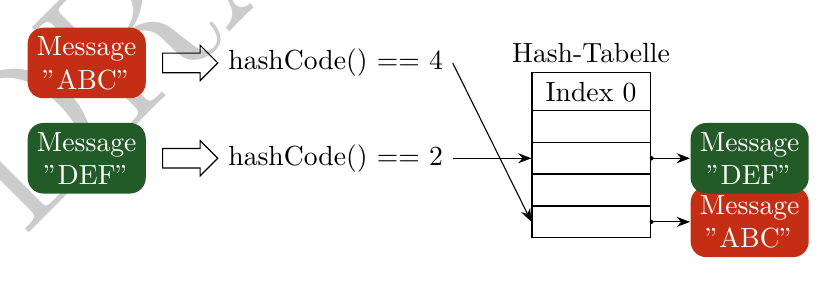
\begin{tikzpicture}
    \begin{scope}[every node/.style={text=white, minimum width=1.5cm, minimum height=0.8cm, rounded corners=2mm, align=center}]
        \node[fill=redcontrast] (abc) at (0,0) {Message\\"ABC"};
        \node[fill=basegreen, below=3mm of abc] (def) {Message\\"DEF"};        
    \end{scope}

    \begin{scope}[every node/.style={single arrow, draw, minimum height=7mm, single arrow head extend=1mm}]
        \node[right=2mm of abc.east] (arr1) {};
        \node[right=2mm of def.east] (arr2) {};        
    \end{scope}

    \node[right=0mm of arr1.east] (hc1) {\lstinline{hashCode() == 4}};
    \node[right=0mm of arr2.east] (hc2) {\lstinline{hashCode() == 2}};

    \matrix[row sep = -0.1mm,matrix anchor=idx3.west, nodes={draw, minimum width=1.5cm, minimum height=0.4cm}, right=1cm of hc2.east]
    {
        \node (idx0) {Index 0}; \\
        \node {}; \\
        \node (idx3) {}; \\
        \node {}; \\
        \node (idx5) {}; \\
    };
    \node[above=0mm of idx0, align=center] {Hash-Tabelle};

    \begin{scope}[>=Stealth]
        \draw[->] (hc1.east) -- (idx5.west);
        \draw[->] (hc2.east) -- (idx3.west);
    \end{scope}

    \begin{scope}[every node/.style={text=white, minimum width=1.5cm, minimum height=0.8cm, rounded corners=2mm, align=center}]
        \node[fill=redcontrast, right=5mm of idx5.east] (abc2) {Message\\"ABC"};
        \node[fill=basegreen, right=5mm of idx3.east] (def2) {Message\\"DEF"};        
    \end{scope}
    \begin{scope}[cbase /.tip={Arc Barb[reversed, line width=1pt, width=2pt, length=1pt]},>=Stealth]
        \draw[{cbase}->] (idx5.east) -- (abc2.west);
        \draw[{cbase}->] (idx3.east) -- (def2.west);
    \end{scope}
\end{tikzpicture}
        \section{Generics}
Generics werden verwendet um einen einheitlichen Elementtypen zu forcieren. Beispielsweise in einer ArrayList.
% TODO: evtl. erwähnen, dass static nicht nötig ist
\subsection{Benennungskonventionen}
\begin{tabularx}{\columnwidth}{@{}l l l@{}}
    \tabitem{}E -- Element & \tabitem{}N -- Number & \tabitem{}V -- Value\\

    \tabitem{}K -- Key &\tabitem{}T -- Type &\tabitem{}S, U, V, \ldots -- 2nd, 3rd, 4th types
\end{tabularx}

\subsection{Generische Typen}
\vspace{-0.8\abovedisplayskip}
\begin{minipage}[t]{0.6\columnwidth}
    \subsubsection{Verschiedene generische Typen}
    \lstinputlisting[morekeywords={Integer}]{snippets/gentyp1.java}
\end{minipage}\hfill%
\begin{minipage}[t]{0.4\columnwidth}
    \subsubsection{Statische Typ-Prüfung}
    \lstinputlisting{snippets/gentyp2.java}
\end{minipage}

\subsubsection{Kein Type-Cast}
\lstinputlisting{snippets/gentyp3.java}

\subsection{Generische Klasse}
\vspace{-0.7\abovedisplayskip}
\begin{minipage}[t]{0.5\columnwidth}
    \subsubsection{Typ-Parameter}
    Platzhalter für generischen Typ.
    \lstinputlisting[escapechar=!]{snippets/genclass1.java}
    \begin{tikzpicture}[remember picture, overlay]
        \draw[semithick, color=bluecontrast,decoration={brace,mirror,raise=1pt}, decorate] (tp1.south) -- node[text=bluecontrast,below=3pt] {Typ-Parameter} (tp2.south);
    \end{tikzpicture}
\end{minipage}\hfill
\begin{minipage}[t]{0.5\columnwidth}
    \subsubsection{Typ-Argument}
    Typ bei Einsatz angeben.
    \lstinputlisting[style=basestyle,numbers=left,xleftmargin=1.2em,escapechar=!]{snippets/genclass2.java}
    \begin{tikzpicture}[remember picture, overlay]
        \draw[semithick, color=redcontrast,decoration={brace,mirror,raise=1pt}, decorate] (ta1.south) -- node[text=redcontrast,below=3pt] {Typ-Argument} (ta2.south);
    \end{tikzpicture}
\end{minipage}

\begin{itemize}
    \item Typ-Parameter dient als "Typ-Variable" innerhalb der generischen Klasse.
    \item Wie normaler Typ verwendbar.
\end{itemize}

\subsection{Generische Methode}

\begin{minipage}[t]{0.5\columnwidth}
    \vspace{-0.8\abovedisplayskip}
    \lstinputlisting{snippets/genmet1.java}
\end{minipage}\hfill%
\begin{minipage}[t]{0.49\columnwidth}
    \raggedright%
    Beim Aufruf generischer Methoden muss der Typ nicht angegeben werden.
\end{minipage}


\subsection{Generische Interfaces}
\subsubsection{Beispiel mit Iterator}
\begin{minipage}[t]{0.5\columnwidth}
    \vspace{-0.7\abovedisplayskip}
    \lstinputlisting{snippets/genint1.java}
\end{minipage}\hfill%
\begin{minipage}[t]{0.5\columnwidth}
    \vspace{-0.7\abovedisplayskip}
    \lstinputlisting{snippets/genint2.java}
\end{minipage}

\subsection{Iteration}
\begin{minipage}[t]{0.32\columnwidth}
    For-Schleife:
    \lstinputlisting{snippets/genericfor1.java}
\end{minipage}\hfill%
\begin{minipage}[t]{0.68\columnwidth}
    Tatsächlich generierter Code:
    \lstinputlisting{snippets/genericfor2.java}
\end{minipage}

\subsection{Type Bounds}
\vspace{-0.8\abovedisplayskip}
\begin{minipage}[t]{0.39\columnwidth}
    \subsubsection{Nutzen}
    \raggedright%
    \begin{itemize}
        \item Typ-Argument \textbf{muss} Subtyp von \lstinline{Graphic} sein
    \end{itemize}
\end{minipage}\hfill%
\begin{minipage}[t]{0.6\columnwidth}
    \subsubsection{Beispiel}
    \lstinputlisting{snippets/gentb1.java}
    Mehrere Bounds können mit \& verknüpft werden.
\end{minipage}
\begin{itemize}
    \item Bei Verwendung von spez. Funktionen innerh.\ generischer Funktion/Klasse
\end{itemize}


% \vfill\null%

% DONE: Generische Methoden
    % DONE: Type Inferenz bei generischen Methoden
% DONE: Generische Interfaces
% DONE: Type Bounds von Parametern
        \section{Exceptions}

% TODO: add some more examples for checked and unchecked exceptions
\begin{minipage}[t]{0.43\columnwidth}
    \subsection{Checked Exceptions}
    \raggedright%
    \begin{itemize}
        \item Bei Methodendeklaration müssen Exceptions angegeben werden, welche gechecked werden müssen.
    \end{itemize}
\end{minipage}\hfill%
\begin{minipage}[t]{0.56\columnwidth}
    \lstinputlisting{snippets/exceptchecked.java}
\end{minipage}
\begin{itemize}
    \item Nach \lstinline{throws} können mehrere Exceptions mit "\lstinline{,}" separiert angegeben werden.
\end{itemize}
\vspace{-0.4\abovedisplayskip}
\begin{minipage}[t]{0.44\columnwidth}
    \subsection{Unchecked Exceptions}
    \raggedright%
    \begin{itemize}
        \item Keine \lstinline{throws}-Deklaration und keine Behandlung nötig
        \item \lstinline{RuntimeException} und \lstinline{Error} sowie Subklassen
        \item Behebung nur durch Änderung des Codes
    \end{itemize}
\end{minipage}\hfill%
\begin{minipage}[t]{0.55\columnwidth}
    \lstinputlisting{snippets/exceptunchecked.java}
\end{minipage}

\vspace{0.3\abovedisplayskip}
\begin{minipage}[t]{0.59\columnwidth}
    \subsection{Exceptions behandeln}
    Werden mit \lstinline{try-catch}-Blöcken behandelt.
    \lstinputlisting{snippets/exceptcatch.java}
\end{minipage}\hfill%
\begin{minipage}[t]{0.4\columnwidth}
    \subsection{Ablauf}
    \begin{minipage}[t]{0.49\columnwidth}
        \subsubsection{Normalfall}
        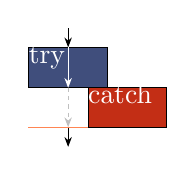
\begin{tikzpicture}[every node/.style={draw, 
            fill=bluecontrast, 
            text=white, 
            text width=1cm, 
            minimum height=3mm,
            inner sep=0mm, 
            text depth=3mm,
            text height=2mm,
            align=flush left}, >={Stealth[length=1.25mm]}]
            \node at (0,-0.5) (try) {try};
            \node[fill=redcontrast,anchor=north west, postaction={draw,thin}, line width=0mm] at ($(try.south)!0.5!(try.south east)$) (catch) {catch};
            \draw[->] (0,0) -- (try.north);
            \draw[white, ->] (try.north) -- (try.south);
            \draw[lightgray, dash pattern=on 1.5pt off 1.5pt, ->] (try.south) -- (try.south |- catch.south);
            \draw[->] (try.south |- catch.south) -- +(0,-0.25);
            \draw[coralcontrast,-] ($(catch.south west)+(-0.2pt,0mm)$) -- (try.south west |- catch.south);
        \end{tikzpicture}
    \end{minipage}\hfill
    \begin{minipage}[t]{0.49\columnwidth}
        \subsubsection{Ausnahmefall}
        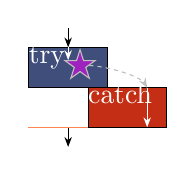
\begin{tikzpicture}[>={Stealth[length=1.25mm]}]
            \begin{scope}[every node/.style={draw, 
                fill=bluecontrast, 
                text=white, 
                text width=1cm, 
                minimum height=3mm,
                inner sep=0mm, 
                text depth=3mm,
                text height=2mm,
                align=flush left}]
                \node at (0,-0.5) (try) {try};
                \node[fill=redcontrast,anchor=north west, postaction={draw,thin}, line width=0mm] at ($(try.south)!0.5!(try.south east)$) (catch) {catch};
            \end{scope}
            \node[fill=claretcontrast, star, star point height=1.235mm, minimum size=4mm, inner sep=0mm, star points=5, draw=lightgray, anchor=inner point 2, xshift=0.7mm] (someexcept) at (try.center) {};
            \draw[lightgray, dash pattern=on 1.5pt off 1.5pt, ->, looseness=0.5] (someexcept) to[out=0,in=90] ($(catch.north)!0.5!(catch.north east)$);
            \draw[->] (0,0) -- (try.north);
            \draw[white, ->] (try.north) -- (try.north |- someexcept.inner point 1);
            \draw[white, ->] ($(catch.north)!0.5!(catch.north east)$) -- ($(catch.south)!0.5!(catch.south east)$);
            \draw[->] (try.south |- catch.south) -- +(0,-0.25);
            \draw[coralcontrast,-] ($(catch.south west)+(-0.2pt,0mm)$) -- (try.south west |- catch.south);
        \end{tikzpicture}
    \end{minipage}
\end{minipage}


\subsection{Stack Unwinding}
\begin{itemize}
    \item Baue solange Methoden-Frames vom Stack ab, bis Exception behandelt wird
    \item Falls \lstinline{main()} mit Exception returnt, behandelt JVM diese mit Programmabbruch
\end{itemize}

% \vfill\null%

\subsection{Error vs. Exception}
\vspace{-.9\abovedisplayskip}
\begin{minipage}[t]{0.5\columnwidth}
    \subsubsection{Error}
    \raggedright%
    \begin{itemize}
        \item Schwerwiegende Fehler, die \textbf{nicht behandelt} werden sollen
        \item Fehler in JVM: \lstinline{OutOfMemoryError}, \lstinline{StackOverflowError} % ChkTeX 13
        \item Programmierfehler: \lstinline{AssertionError}
    \end{itemize}
\end{minipage}\hfill%
\begin{minipage}[t]{0.49\columnwidth}
    \subsubsection{Exception}
    \raggedright%
    \begin{itemize}
        \item Laufzeitfehler, die \textbf{behandelbar} sind
        \item Fehler in Eingabe, Parameter, Bedienung, \ldots z.B. \lstinline{IOException} \textrightarrow{} grundsätzlich behandeln
        \item Andere Laufzeitfehler \textrightarrow{} lieber nicht behandeln
    \end{itemize}
\end{minipage}
    
\subsection{\textsf{\textbf{\textcolor{keywordcolour}{finally}}}-Ablauf}
\vspace{-.9\abovedisplayskip}
\begin{minipage}[t]{0.33\columnwidth}
    \subsubsection{Keine Exception}
    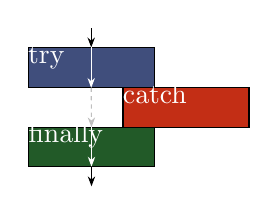
\begin{tikzpicture}[every node/.style={draw, 
        fill=bluecontrast, 
        text=white, 
        text width=1.6cm, 
        minimum height=3mm,
        inner sep=0mm, 
        text depth=3mm,
        text height=2mm,
        align=flush left}, >={Stealth[length=1.25mm]}]
        \node at (0,-0.5) (try) {try};
        \node[fill=redcontrast,anchor=north west, postaction={draw,thin}, line width=0mm] at ($(try.south)!0.5!(try.south east)$) (catch) {catch};
        \node[fill=basegreen, anchor=north east, postaction={draw,thin}, line width=0mm] at ($(catch.south)!0.5!(catch.south west)$) (finally) {finally};
        \draw[->] (0,0) -- (try.north);
        \draw[white, ->] (try.north) -- (try.south);
        \draw[lightgray, dash pattern=on 1.5pt off 1.5pt, ->] (try.south) -- (finally.north);
        \draw[white, ->] (finally.north) -- (finally.south);
        \draw[->] (finally.south) -- +(0,-0.25);
    \end{tikzpicture}
\end{minipage}
\begin{minipage}[t]{0.33\columnwidth}
    \subsubsection{Behandelte Exception}
    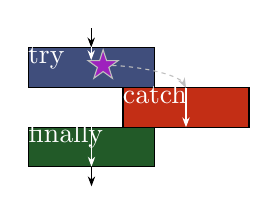
\begin{tikzpicture}[>={Stealth[length=1.25mm]}]
        \begin{scope}[every node/.style={draw, 
            fill=bluecontrast, 
            text=white, 
            text width=1.6cm, 
            minimum height=3mm,
            inner sep=0mm, 
            text depth=3mm,
            text height=2mm,
            align=flush left}]
            \node at (0,-0.5) (try) {try};
            \node[fill=redcontrast,anchor=north west, postaction={draw,thin}, line width=0mm] at ($(try.south)!0.5!(try.south east)$) (catch) {catch};
            \node[fill=basegreen, anchor=north east, postaction={draw,thin}, line width=0mm] at ($(catch.south)!0.5!(catch.south west)$) (finally) {finally};
        \end{scope}
        \node[fill=claretcontrast, star, star point height=1.235mm, minimum size=4mm, inner sep=0mm, star points=5, draw=lightgray, anchor=inner point 2, xshift=0.7mm] (someexcept) at (try.center) {};
        \draw[lightgray, dash pattern=on 1.5pt off 1.5pt, ->, looseness=0.5] (someexcept) to[out=0,in=90] (catch.north);
        \draw[->] (0,0) -- (try.north);
        \draw[white, ->] (try.north) -- (try.north |- someexcept.inner point 1);
        \draw[white, ->] (catch.north) -- (catch.south);
        \draw[white, ->] (finally.north) -- (finally.south);
        \draw[->] (finally.south) -- +(0,-0.25);
    \end{tikzpicture}
\end{minipage}\hfill%
\begin{minipage}[t]{0.33\columnwidth}
    \subsubsection{Unbehandelte Exception}
    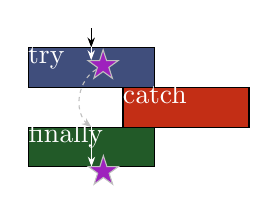
\begin{tikzpicture}[>={Stealth[length=1.25mm]}]
        \begin{scope}[every node/.style={draw, 
            fill=bluecontrast, 
            text=white, 
            text width=1.6cm, 
            minimum height=3mm,
            inner sep=0mm, 
            text depth=3mm,
            text height=2mm,
            align=flush left}]
            \node at (0,-0.5) (try) {try};
            \node[fill=redcontrast,anchor=north west, postaction={draw,thin}, line width=0mm] at ($(try.south)!0.5!(try.south east)$) (catch) {catch};
            \node[fill=basegreen, anchor=north east, postaction={draw,thin}, line width=0mm] at ($(catch.south)!0.5!(catch.south west)$) (finally) {finally};
        \end{scope}
        \node[fill=claretcontrast, star, star point height=1.235mm, minimum size=4mm, inner sep=0mm, star points=5, draw=lightgray, anchor=inner point 2, xshift=0.7mm] (someexcept) at (try.center) {};
        \draw[lightgray, dash pattern=on 1.5pt off 1.5pt, ->] (someexcept) to[out=-150,in=150] (finally.north);
        \draw[->] (0,0) -- (try.north);
        \draw[white, ->] (try.north) -- (try.north |- someexcept.inner point 1);
        \draw[white, ->] (finally.north) -- (finally.south);
        \node[fill=claretcontrast, star, star point height=1.235mm, minimum size=4mm, inner sep=0mm, star points=5, draw=lightgray, anchor=inner point 2, xshift=0.7mm, yshift=-0.88mm] at (finally.south) {};
    \end{tikzpicture}
\end{minipage}
\lstinline{finally}-Block wird immer ausgeführt, auch wenn \lstinline{catch}-Block eine Exception wirft.

% \vspace{1ex}
\begin{minipage}[t]{0.6\columnwidth}
    \subsection{try-with-resources}
    \begin{itemize}
        \item Objekte, die geschlossen werden müssen
        \item \lstinline{AutoCloseable}-Interface
    \end{itemize}
    \lstinputlisting{snippets/excepttrywith.java}
    \subsection{Benutzerdefinierte Exceptions}
    \lstinputlisting{snippets/exceptcustom.java}
\end{minipage}\hfill%
\begin{minipage}[t]{0.39\columnwidth}
    \subsection{Throwable}
    \raggedright%
    \begin{itemize}
        \item Klasse oder Unterklasse von \lstinline{Throwable}
        \item Klassifizierung des Fehlers
    \end{itemize}
    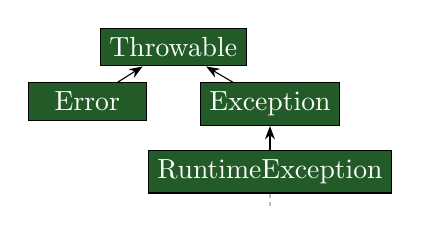
\begin{tikzpicture}[baseline=(current bounding box.north), 
        every node/.style={
            draw, 
            fill=basegreen,
            text=white,
            minimum width=1.5cm,
            minimum height=4.5mm,
            align=center},
        >={Stealth}]

        \node[](throwable) at (0,0) {Throwable};
        \node[below left=2mm and -6mm of throwable](error) {Error};
        \node[below right=2mm and -6mm of throwable](exception) {Exception};
        \node[below=3mm of exception] (runtime) {RuntimeException};
        \draw[->] (error) -- (throwable);
        \draw[->] (exception) -- (throwable);
        \draw[->] (runtime) -- (exception);
        \draw[lightgray, dash pattern=on 1.5pt off 1.5pt, -] (runtime.south) -- +(0,-2mm);  
    \end{tikzpicture}
\end{minipage}

        \section{Lambdas}

\subsection{Syntax}
\lstinputlisting[style=basestyle, escapechar=!, basicstyle=\sffamily, numbers=left, xleftmargin=1em]{snippets/lambdasyntax.java}
% \raggedright%
\begin{itemize}
    \item Parameter als Parameterlist übergeben \lstinline{@(p1,p2,...)@}
    \item \lstinline{return} benötigt in Methodenkörper, wenn \lstinline|{}| verwendet
    \item \lstinline{return}-typ implizit
    \item Wenn nur ein Statement, dann \lstinline|{}| und \lstinline{return} optional
\end{itemize}
% \begin{minipage}[t]{0.35\columnwidth}
% \end{minipage}\hfill%
% \begin{minipage}[t]{0.64\columnwidth}
\subsection{Beispiel}
\lstinputlisting{snippets/lambda.java}
% \end{minipage}
        \section{Unit Tests}

\begin{minipage}[t]{0.65\columnwidth}
    \subsection{Konzept}
    \begin{itemize}
        \item Test von abgenzbarem Programmteil (Unit)
        \item Regressionstest: hat eine Änderung die bestehenden Funktionen geschädigt?
    \end{itemize}
\end{minipage}\hfill%
\begin{minipage}[t]{0.31\columnwidth}
    \subsection{Blackbox-Test}
    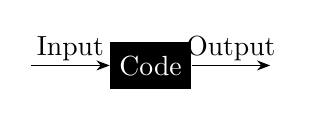
\begin{tikzpicture}[>=Stealth]
        \node[minimum height=6mm, fill=black, text=white] (bbox) at (0,0) {Code};
        \draw[<-] (bbox.west) -- ++(-1,0) node[midway, above=-0.7mm] {Input};
        \draw[->] (bbox.east) -- ++(1,0) node[midway, above=-0.7mm] {Output};
    \end{tikzpicture}
\end{minipage}
\vspace{-0.5\abovedisplayskip}
\begin{center}
    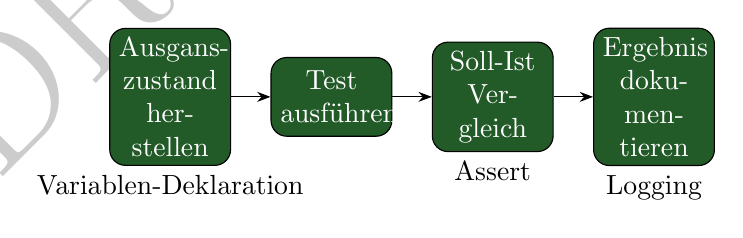
\begin{tikzpicture}[every node/.style={draw=black, 
        fill=basegreen, 
        text=white, 
        text width=1.3cm, 
        rounded corners=0.2cm,
        minimum height=1cm,
        align=center},
        >=Stealth]
        \node (1) at (0,0) {Ausgans- zustand herstellen};
        \node[right=5mm of 1] (2) {Test ausführen};
        \node[right=5mm of 2] (3) {Soll-Ist Vergleich};
        \node[right=5mm of 3] (4) {Ergebnis dokumentieren};
        \draw[->] (1) -- (2);
        \draw[->] (2) -- (3);
        \draw[->] (3) -- (4);
        \begin{scope}[every node/.style={text=black, minimum height=0, fill=none, draw=none}]
            \node[below=0mm of 1] {Variablen-Deklaration};
            \node[below=0mm of 3] {Assert};
            \node[below=0mm of 4] {Logging};
        \end{scope}
    \end{tikzpicture}
\end{center}
\vspace{-1.3\abovedisplayskip}


\subsection{Äquivalenzklassenbildung}
\vspace{-0.8\abovedisplayskip}
\begin{minipage}[t]{0.5\columnwidth}
    \subsubsection{1. Klassen bilden}
    \raggedright%
    Wertebereich der Parameter in Bereiche zerlegen, die von der Funktion wahrscheinlich gleich behandelt werden.
\end{minipage}\hfill%
\begin{minipage}[t]{0.49\columnwidth}
    \subsubsection{2. Tests erstellen}
    \raggedright%
    Pro Äquivalenzklasse Belegung der Eingangsvariablen wählen und Testfall schreiben.
\end{minipage}

\subsection{Aufbau Testmethode}
\begin{minipage}[t]{0.65\columnwidth}
    \vspace{-0.8\abovedisplayskip}
    \lstinputlisting{snippets/archunit.java}
\end{minipage}\hfill%
\begin{minipage}[t]{0.34\columnwidth}
    \raggedright%
    \begin{itemize}
        \item Keine Parameter
        \item Rückgabetyp \lstinline{void}
        \item \lstinline{¦¦@Test}-Annotation
        \item Asserts um Werte zu prüfen
        \item Testmethoden isoliert von anderen Testmethoden
    \end{itemize}
\end{minipage}

\subsection{Asserts}
\begin{minipage}[t]{0.54\columnwidth}
    \subsubsection{Prüfen von Gleichheit (inhaltlich)}
    \begin{itemize}
        \item \lstinline{assertEquals(expected, actual)}
        \item \lstinline{assertArrayEquals(expected, actual)}
        \item \ldots
    \end{itemize}
\end{minipage}\hfill%
\begin{minipage}[t]{0.45\columnwidth}
    \subsubsection{Prüfen von boolschen Ausdrücken}
    \begin{itemize}
        \item \lstinline{assertTrue(actual)}
        \item \lstinline{assertFalse(actual)}
        \item \ldots
    \end{itemize}
\end{minipage}

\subsection{FIRST-Prinzip}
\begin{tabular}{@{\hspace{1.3mm}}l l@{}}
    \tabitem\textbf{\cgn{F}}ast: &Ausführung ist schnell\\
    \tabitem\textbf{\cgn{I}}ndependent: &Reihenfolge der Tests ist nicht relevant.\\
    \tabitem\textbf{\cgn{R}}epeatable: &Ergebnis ändert sich nur wenn sich Implementierung ändert.\\
    \tabitem\textbf{\cgn{S}}elf-validating: &Testergebnis benötigt keine Interpretation.\\
    \tabitem\textbf{\cgn{T}}imely: &Tests werden früh geschrieben.
\end{tabular}

        \section{Stream-API}


\begin{minipage}[t]{0.6\columnwidth}
    \begin{itemize}
        \item Für deklarative Verarbeitung von Datenströmen
        \item Definiere \textbf{was} gemacht werden soll, nicht \textbf{wie}
    \end{itemize}
    \subsection{Beispiel}
    \lstinputlisting{snippets/streamapiex.java}
\end{minipage}\hfill%
\begin{minipage}[t]{0.39\columnwidth}
    \begingroup
    % change \section command temporarily to be centered
    \titleformat{\subsection}
            {\fontsize{9}{8}\selectfont\bfseries\filcenter}
            {\thesubsection}
            {0mm}
            {\phantomsection\myul{#1}} % \phantomsection to make hyperref link to correct section
    \subsection{Idee}
    \endgroup
    \begin{center}
        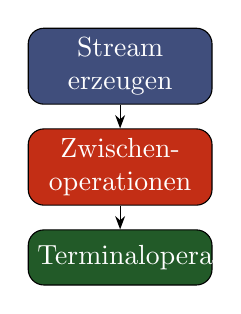
\begin{tikzpicture}[every node/.style={
            draw, 
            text=white, 
            rounded corners=2mm,
            minimum width=2.1cm,
            text width=2.1cm,
            minimum height=7mm, 
            align=center},
            >=Stealth]
            \node[fill=bluecontrast] (a) at (0,0) {Stream erzeugen};
            \node[fill=redcontrast, below=3mm of a] (b) {Zwischen- operationen};
            \node[fill=basegreen, below=3mm of b] (c) {Terminaloperation};
            \draw[->] (a) -- (b);
            \draw[->] (b) -- (c);
        \end{tikzpicture}
    \end{center}
\end{minipage}



\subsection{Endliche Quellen}
\begin{tabular}{@{\hspace{1.3mm}}ll@{}}
    \tabitem\mylstbox{IntStream.range(0, 10)}: &Zahlen von 0 bis 9\\
    \tabitem\mylstbox{Stream.of(2, 3, 4)}: &Eigene Aufzählung\\
    \tabitem\mylstbox{Stream.empty()}: &Leerer Stream\\
    \tabitem\mylstbox{Collection.stream()}: &Stream aus Collection\\
    \tabitem\mylstbox{Stream.concat(s1, s2)}: &Verkettung zweier Streams
\end{tabular}

\subsection{Unendliche Quellen}
\vspace{-0.7\baselineskip}
\begin{minipage}[t]{0.5\columnwidth}
    \subsubsection{\textsf{generate()}}
    \lstinputlisting{snippets/streamgenerate.java}
\end{minipage}\hfill%
\begin{minipage}[t]{0.49\columnwidth}
    \subsubsection{\textsf{iterate()}}
    \lstinputlisting{snippets/streamiterate.java}
\end{minipage}

\subsection{Zwischenoperationen}
\begin{minipage}[t]{\columnwidth}
    \raggedright%
    Bei Collections ist es \textbf{nicht} erlaubt, diese mit Zwischenoperationen zu ändern. Auch nicht erlaubt sind Abhängigkeiten zu äusseren, änderbaren Variablen.
\end{minipage}
\begin{tabular}{@{\hspace{1.3mm}}l@{\hspace{1mm}}l@{}}
    \tabitem\mylstbox{filter(Predicate)}: &Filtern mit Predicate-Funktionsobjekt/Lambda\\
    \tabitem\mylstbox{map(Function)}: &Projizieren mit Funktionsobjekt/Lamda\\
    \tabitem\mylstbox{mapToInt...(Function)}: &Projizieren auf \lstinline|int|, \lstinline|long|, \lstinline|double|\\
    \tabitem\mylstbox{sorted()}: &Sortieren mit/ohne Comparator\\
    \tabitem\mylstbox{distinct()}: &Duplikate entfernen (\lstinline|equals()|)\\
    \tabitem\mylstbox{limit(long n)}: &n-Elemente liefern\\
    \tabitem\mylstbox{skip(long n)}: &n-Elemente überspringen
\end{tabular}
\vfill\null%

\subsection{Terminaloperationen}
\begin{tabular}{@{\hspace{1.3mm}}l@{\hspace{1mm}}l@{}}
    \tabitem\mylstbox{forEach(Consumer)}: &Pro Element Operation anwenden, meist mit Seiteneffekt\\
    \tabitem\mylstbox{count()}: &Anzahl Elemente\\
    \tabitem\mylstbox{min()}, \mylstbox{max()}: &Mit Comparator-Argument\\
    \tabitem\mylstbox{average()}, \mylstbox{sum()}: &Nur für numerische Streams\\
    \tabitem\mylstbox{findAny()}, \mylstbox{findFirst()}: &Gibt irgendein / erstes Element zurück
\end{tabular}


\subsection{Optional-Wrapper}
\begin{itemize}
    \item Wert exisitiert oder nicht
    \item \lstinline{average()}, \lstinline{min()}, \lstinline{max()} geben \lstinline{Optional} zurück
    \item Überprüfung mit \lstinline{isPresent()}
\end{itemize}


\subsection{Matching}
\begin{itemize}
    \item \lstinline{allMatch()}, \lstinline{anyMatch()}, \lstinline{noneMatch()}
    \item Prüfen ob Prädikat auf alle/irgendein/kein Element zutrifft
\end{itemize}


\subsection{Lazy Evaluation}
\begin{itemize}
    \item Element wird erst bereitgestellt, wenn Nachfolger Element anfordert
    \item Unendliche Streams sind meist Lazy
\end{itemize}


\subsection{Collectors}
\begin{tabular}{@{\hspace{1.3mm}}l@{\hspace{1mm}}l@{}}
    \tabitem\mylstbox{Collectors.toList()}: &Liste aller Elemente\\
    \tabitem\mylstbox{Collectors.toCollection(TreeSet::new)}: &In beliebige Collection abbilden\\
    \tabitem\mylstbox{Collectors.groupingBy(key, aggregator)}: &Gruppierung, Aggregator optional\\
    \multicolumn{2}{l}{\phantom{\tabitem}Aggregator: (\lstinline|averaging|, \lstinline|summing|, \lstinline|counting|)}
\end{tabular}


\subsection{Gruppierungen}
\lstinputlisting[morekeywords={Integer}]{snippets/streamgrouping1.java}
\lstinputlisting[morekeywords={Integer}]{snippets/streamgrouping2.java}
        \section{Input/Output}
% DONE: rename to Input/Output
% DONE: Byte Streams
% DONE: Character Stream
% DONE: File I/O
    % DONE: Zeilenweise lesen
% TODO: Wichtige Methoden
% DONE: Standard I/O
    % DONE: Zeilenweise lesen 
% TODO: Klassenhierarchie
% TODO: Exceptions
% TODO: "einfachste Zugriffe"

\subsection{Streams allgemein}
\vspace{-0.7\abovedisplayskip}
\begin{minipage}[t]{0.5\columnwidth}
    \subsubsection{Input Stream}
    \begin{itemize}
        \item Daten \textbf{von aussen} lesen
        \item Tastatur, Netzwerk, Dateien, \ldots
    \end{itemize}
\end{minipage}\hfill%
\begin{minipage}[t]{0.49\columnwidth}
    \subsubsection{Output Stream}
    \begin{itemize}
        \item Daten \textbf{nach aussen} schreiben
        \item Bildschirm, Netzwerk, Dateien, \ldots
    \end{itemize}
\end{minipage}

\begin{minipage}[t]{0.5\columnwidth}
    \subsection{Byte Streams}
    \raggedright%
    \begin{itemize}
        \item Byteweises lesen (8-Bit Daten)
        \item Erben von: \lstinline{InputStream}, \lstinline{OutputStream}
        \item Beispiel: \lstinline{FileInputStream}, \lstinline{FileOutputStream}
        \item Close bei Exceptions: \lstinline{in.close()} in \lstinline{finally}-Block
    \end{itemize}
\end{minipage}\hfill%
\begin{minipage}[t]{0.49\columnwidth}
    \subsection{Character Streams}
    \raggedright%
    \begin{itemize}
        \item Unicode mit 16-Bit (UTF-16) codiert
        \item Erben von: \lstinline{Reader}, \lstinline{Writer}
        \item Zeichen-/Zeilenweise Ein- \& Ausgabe
    \end{itemize}
\end{minipage}


\subsubsection{\textsf{InputStream}}
\lstinputlisting{snippets/inputstream.java}
\begin{itemize}
    \item Lese \lstinline{length} Bytes in Array \lstinline{b} ab Index \lstinline{offset}
    \item Rückgabe = gelesene Bytes (-1 \textlrarrow{} end of stream)
\end{itemize}

\subsubsection{\textsf{OutputStream}}
\lstinputlisting{snippets/outputstream.java}
\begin{itemize}
    \item Schreibt eventuell noch im Cache zwischengespeicherte Ausgaben
    \item Implizit bei \lstinline{close()}
\end{itemize}

\subsection{File-Input}
% \subsubsection{Beispiel}
\vspace{-0.7\abovedisplayskip}
\begin{minipage}[t]{0.6\columnwidth}
    \lstinputlisting[escapechar=!]{snippets/fileinput.java}
\end{minipage}\hfill%
\begin{minipage}[t]{0.39\columnwidth}
    \begin{tikzpicture}[
        every node/.style={
            align=center,
            minimum width=2cm,
            minimum height=8mm,
            draw,
            rounded corners=2mm},
        every path/.style={
            rounded corners=2pt},
        remember picture, 
        overlay,
        >=Stealth]
        \node[text width=2.2cm, right=1.7cm of fileinnew] (fintxt) {Bestehende Datei zum Lesen öffnen};
        \node[below=2mm of fintxt] (eof) {-1: end of file};
        \node[text width=2cm, below=2mm of eof] (read) {Gelesenes Byte (wenn positiv)};
        \draw[->] (fintxt.west) -- (fileinnew.east);
        \draw[->] (eof.west) -- ++(-1cm,0) |- (fileineof.east);
        \draw[->] (read.west) -- ++(-1.5cm,0) |- (fileinread.east);
    \end{tikzpicture}
\end{minipage}

\subsection{File-Output}
% \subsubsection{Beispiel}
\vspace{-0.7\abovedisplayskip}
\begin{minipage}[t]{0.6\columnwidth}
    \lstinputlisting[escapechar=!]{snippets/fileoutput.java}
\end{minipage}\hfill%
\begin{minipage}[t]{0.39\columnwidth}
    \begin{tikzpicture}[
        every node/.style={
            align=center,
            minimum width=2cm,
            minimum height=8mm,
            draw,
            rounded corners=2mm},
        every path/.style={
            rounded corners=2pt},
        remember picture, 
        overlay,
        >=Stealth]
        \node[text width=2.2cm] (fouttxt) at (fileoutnew.east -| fintxt.south) {Datei neu andlegen bzw. überschreiben};
        \node[text width=2cm] (foutappend) at (fileoutappend.east -| fouttxt.south) {An Datei anhängen, falls existiert};
        \node[text width=3cm] (foutclose) at ($(fouttxt.south)!0.5!(foutappend.north)$) {Schreiben des Rests beim Schliessen ("Flush")};
        \draw[->] (fouttxt.west) -- (fileoutnew.east);
        \draw[->] (foutclose.west) -- ++(-1cm,0) |- (fileoutclose.east);
        \draw[->] (foutappend.west) -- (fileoutappend.east);
    \end{tikzpicture}
\end{minipage}


\subsection{Einfachster Dateizugriff}

\begin{minipage}[t]{0.67\columnwidth}
    Ganze Datei binär einlesen:
    \lstinputlisting[escapechar=!]{snippets/fileinput2.java}
\end{minipage}\hfill%
\begin{minipage}[t]{0.32\columnwidth}
    \begin{tikzpicture}[
        every node/.style={
            align=center,
            minimum width=2.5cm,
            text width=2.5cm,
            minimum height=8mm,
            draw,
            rounded corners=2mm},
        every path/.style={
            rounded corners=2pt},
        remember picture, 
        overlay,
        >=Stealth]
        \node (readall) at ($(fileinreadall.south -| fintxt.south)+(0,-3mm)$) {Speicherintensiv bei grossen Dateien};
        \draw[->] (readall.west) -| (fileinreadall.south);
    \end{tikzpicture}
\end{minipage}
    
\vspace{3mm}
\begin{minipage}[t]{0.48\columnwidth}
    Ganze Datei binär schreiben:
    \lstinputlisting{snippets/fileoutput2.java}
\end{minipage}

\subsection{Standard I/O}
\vspace{-0.7\abovedisplayskip}
\begin{minipage}[t]{0.4\columnwidth}
    \subsubsection{\textsf{System.in}}
    \begin{itemize}
        \item \lstinline{InputStream}
    \end{itemize}
\end{minipage}\hfill%
\begin{minipage}[t]{0.59\columnwidth}
    \subsubsection{\textsf{System.out} und \textsf{System.err}}
    \begin{itemize}
        \item \lstinline{PrintStream} (Subklasse von \lstinline{OutputStream})
    \end{itemize}
\end{minipage}

\subsection{File-Reader}
\begin{minipage}[t]{0.55\columnwidth}
    \vspace{-0.8\abovedisplayskip}
    \lstinputlisting{snippets/filereader.java}
\end{minipage}
\begin{minipage}[t]{0.44\columnwidth}
    \raggedright%
    \begin{itemize}
        \item Systemabhängiges Character Set
        \item \lstinline{val = -1} \textrightarrow{} end of file
        \item value ist 16-Bit Unicode char
    \end{itemize}
\end{minipage}
\subsection{File-Writer}
\begin{minipage}[t]{0.6\columnwidth}
    \vspace{-0.8\abovedisplayskip}
    \lstinputlisting{snippets/filewriter.java}
\end{minipage}
\begin{minipage}[t]{0.39\columnwidth}
    \raggedright%
    \begin{itemize}
        \item \lstinline{true} \textrightarrow{} append
        \item \lstinline{.write("")} String schreiben
        \item \lstinline{.write('')} Einzelnen char schreiben
    \end{itemize}
\end{minipage}

\subsection{Zeilenweise lesen (\textcolor{coralcontrast}{\textsf{InputStream}})}
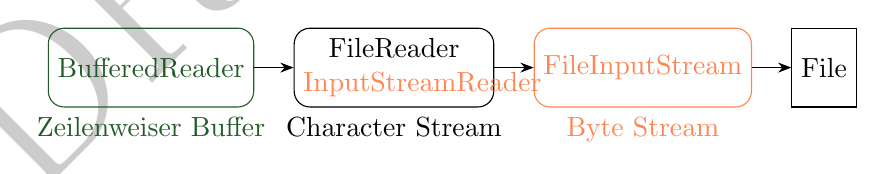
\begin{tikzpicture}[
    every node/.style={
    align=center,
    minimum width=8mm,
    minimum height=1cm,
    draw,
    rounded corners=2mm},
    >=Stealth]
    \node[text=basegreen, draw=basegreen] (br1) at (0,0) {BufferedReader};
    \node[text width=2.3cm, right=0.5cm of br1] (fr1) {FileReader\\ \textcolor{coralcontrast}{InputStreamReader}};
    \node[draw=coralcontrast, text=coralcontrast, right=0.5cm of fr1] (fis1) {FileInputStream};
    \node[rounded corners=0mm, right=0.5cm of fis1] (f1) {File};
    \begin{scope}[
        every node/.style={
            text depth=0pt, 
            anchor=base,
            draw=none}]
        \node[text=basegreen, below=0mm of br1] (brst) {Zeilenweiser Buffer};
        \node[below=0mm of fr1] (frst) {Character Stream};
        \node[text=coralcontrast, below=0mm of fis1] (fisst) {Byte Stream};
    \end{scope}
    \draw[->] (br1) -- (fr1);
    \draw[->] (fr1) -- (fis1);
    \draw[->] (fis1) -- (f1);
\end{tikzpicture}

% \vfill\null%
        \section{Strings}

\begin{tabular}{@{}l l@{}}
    \textbf{Methode} & \textbf{Beschreibung}\\\hhline{==}
    \lstinline|charAt(int idx)| & Zeichen an Position \lstinline|idx|\\\hhline{--}
    \lstinline|length()| & Länge des Strings\\\hhline{--}
    \lstinline|substring(int start, int end)| & Teilstring von \lstinline|start| bis \lstinline|end|\\\hhline{--}
    \lstinline|indexOf(String s)| & Position des ersten Vorkommens von \lstinline|s|\\\hhline{--}
    \lstinline|lastIndexOf(String s)| & Position des letzten Vorkommens von \lstinline|s|\\\hhline{--}
    \lstinline|compareToIgnoreCase(String s)| & Vergleicht Strings (returnt 0 bei Gleichheit)\\\hhline{--}
    \lstinline|isEmpty()| & Returnt \lstinline|true|, wenn String leer ist\\\hhline{--}
    \lstinline|replace("tgt", "rep")| & Ersetzt alle Vorkommen von \lstinline|tgt| mit \lstinline|rep|\\\hhline{--}
    \lstinline|split(String regex)| & Teilt String anhand von \lstinline|regex|\\\hhline{--}
    \lstinline|join("-", "a", "b")| & Verbindet Strings mit \lstinline|"-"| zu \lstinline|"a-b"|\\
\end{tabular}

\subsection{String zu Stream}
\lstinputlisting{snippets/stringstream.java}

	\end{multicols*}
\end{document}